\documentclass[conference]{IEEEtran}
\IEEEoverridecommandlockouts
% The preceding line is only needed to identify funding in the first footnote. If that is unneeded, please comment it out.
%Template version as of 6/27/2024

\usepackage[utf8]{inputenc}
\usepackage[T1]{fontenc}
\usepackage[spanish]{babel}
\usepackage{cite}
\usepackage{amsmath,amssymb,amsfonts}
\usepackage{algorithmic}
\usepackage{graphicx}
\usepackage{textcomp}
\usepackage{xcolor}
\usepackage{hyperref}
\def\BibTeX{{\rm B\kern-.05em{\sc i\kern-.025em b}\kern-.08em
    T\kern-.1667em\lower.7ex\hbox{E}\kern-.125emX}}
\begin{document}

\title{Steam Database: Analisis exploratorio y preprocesamiento
}

\author{\IEEEauthorblockN{1\textsuperscript{ro} David Felipe Marin Rosas}
  \IEEEauthorblockA{\textit{Facultad de Ingeniería} \\
    \textit{Universidad Nacional De Colombia}\\
    Bogotá, Colombia \\
    dmarinro@unal.edu.co}
  \and
  \IEEEauthorblockN{2\textsuperscript{do} Gian Emanuel Morales González}
  \IEEEauthorblockA{\textit{Facultad de Ingeniería} \\
    \textit{Universidad Nacional De Colombia}\\
    Bogotá, Colombia \\
    gimoralesg@unal.edu.co}
  \and
  \IEEEauthorblockN{3\textsuperscript{ro} Juan Felipe Bejarano Salazar}
  \IEEEauthorblockA{\textit{Facultad de Ingeniería} \\
    \textit{Universidad Nacional De Colombia}\\
    Bogotá, Colombia \\
    jbejaranos@unal.edu.co}
  \and
  \IEEEauthorblockN{4\textsuperscript{to} Luis Esteban León Rojas}
  \IEEEauthorblockA{\textit{Facultad de Ingeniería} \\
    \textit{Universidad Nacional De Colombia}\\
    Bogotá, Colombia \\
    luleonr@unal.edu.co}
}

\maketitle

\begin{abstract}
This document details the exploratory data analysis and preprocessing of the ``Steam Games Dataset'', which contains information from over 120,000 video games published on the Steam platform. The objective is to analyze its features (prices, concurrent players, reviews, genres) to build a clean and ready-to-use dataset for predictive models. Through visualizations and robust statistical measures, it was identified that the market exhibits a strong asymmetry: there is a vast number of low-impact free games compared to a small number of massive hits. These findings guided the data cleaning process, null value handling, and feature engineering, setting the groundwork to predict the commercial success of future video games in a structured manner.
\end{abstract}

\begin{IEEEkeywords}
  videojuegos, análisis exploratorio, preprocesamiento, steam database, python, pandas, matplotlib, seaborn, patrones de compra, tendencias de juego, comportamiento del consumidor
\end{IEEEkeywords}

\section{Introducción}

En la última década, la industria de los videojuegos ha experimentado un crecimiento exponencial, consolidándose como uno de los sectores de entretenimiento más lucrativos a nivel global. Dentro de este ecosistema, Steam, operada por Valve Corporation, se mantiene como la plataforma de distribución digital dominante para PC. Con miles de títulos lanzados anualmente, la plataforma genera un volumen masivo de datos que reflejan tendencias de consumo, estrategias de precios y preferencias de género.

El presente documento se centra en el estudio del "Steam Games Dataset", una recopilación de datos a partir de la API ofrecida por steam. Este conjunto de datos captura la diversidad del catálogo de Steam, permitiendo observar desde grandes producciones AAA hasta el emergente mercado de juegos independientes (Indie).

\section{Objetivo}


Analizar qué variables del conjunto de datos influyen más en el éxito de un videojuego. Para este estudio, nuestras tres variables esenciales y métricas de éxito serán: el porcentaje de reseñas positivas categorizado (indicando cantidad total y la razón de aprobación), el número de ventas (\textit{Estimated owners}), y la cantidad de jugadores simultáneos (\textit{Peak CCU}). Con esto, se busca sentar las bases para crear modelos predictivos que estimen el éxito comercial de futuros desarrollos y descubrir qué características se necesitan para triunfar dentro de nichos específicos de mercado.

\section{Descripción del conjunto de datos}
Se utilizó el ``Steam Games Dataset'' \cite{steamDataset}, obtenido a partir de la API oficial de Steam. Este \textit{dataset} cuenta con 122\,611 registros, correspondientes cada uno a un videojuego único, y está compuesto por 39 variables originales.

Las variables abarcan diferentes tipos (ver Figura \ref{fig:dist_vars}): nominales absolutas como el identificador (\textit{AppID}) y nombre (\textit{Name}); de razón para características continuas como el precio (\textit{Price}) y la máxima cantidad de jugadores simultáneos (\textit{Peak CCU}); ordinales como la estimación de compradores (\textit{Estimated owners}); y variables con múltiples valores nominales, como los géneros (\textit{Genres}) y categorías (\textit{Categories}).

\begin{figure}[htbp]
  \centerline{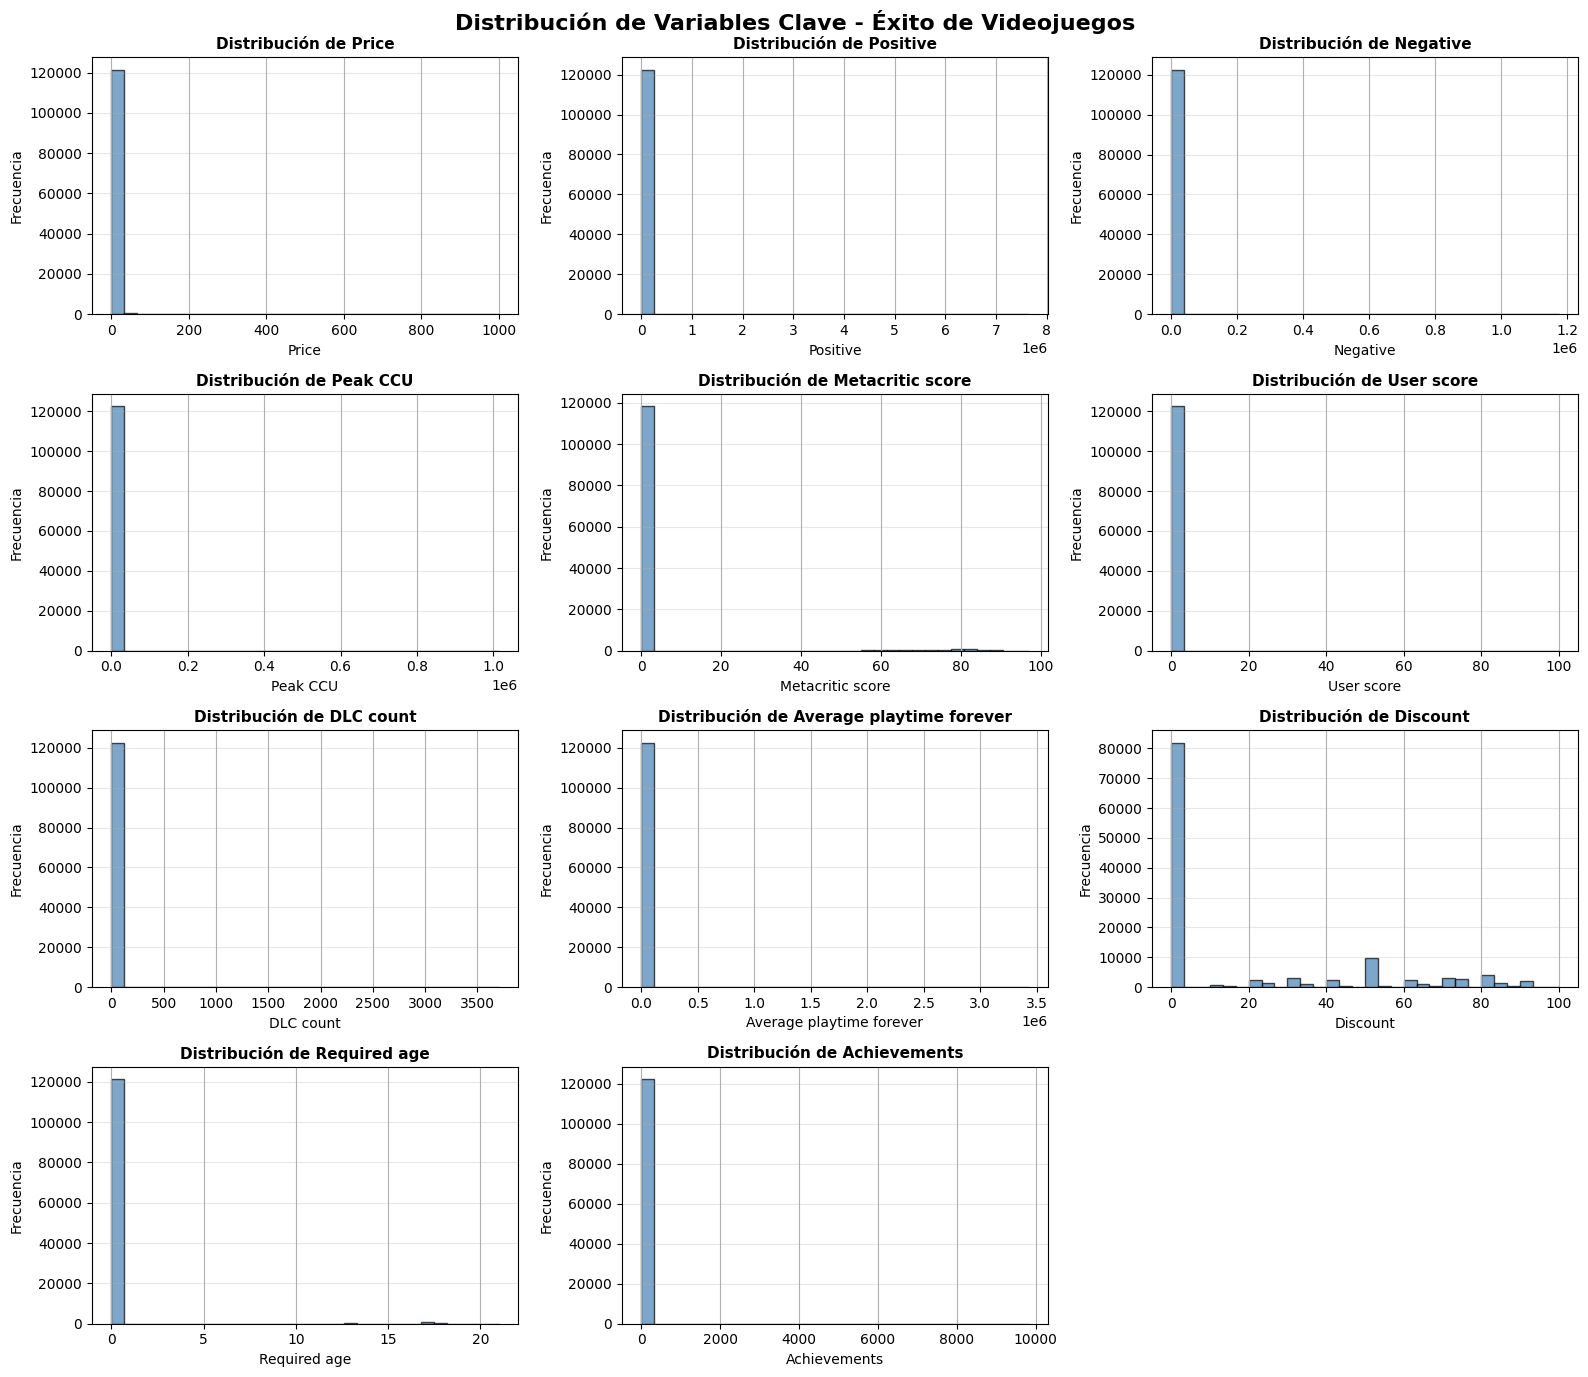
\includegraphics[width=\linewidth]{figures/grafica_1.png}}
  \caption{Distribución de frecuencias para las variables numéricas de Steam. Se evidencia una gran asimetría hacia el lado izquierdo.}
  \label{fig:dist_vars}
\end{figure}

\section{Análisis Exploratorio y Resultados}

\subsection{Análisis de Frecuencias y Medidas de Centralidad}
En la exploración inicial, se observó que casi todos los juegos son compatibles con Windows, superando ampliamente a los desarrollos para Mac y Linux. Al revisar variables numéricas como el precio y el máximo de jugadores activos (\textit{Peak CCU}), se evidenció que una porción muy pequeña de títulos acumula la gran mayoría de las cifras. Al existir tantos valores en cero o muy bajos, existe una enorme diferencia entre el promedio (media aritmética) y la mediana. Para mitigar el efecto de estos valores atípicos (\textit{outliers}), se calculó la \textbf{media truncada} (\textit{trimmed mean}), eliminando el 10\% de los datos más extremos de cada lado para obtener el comportamiento de un juego más ``típico''.

\begin{figure}[htbp]
  \centerline{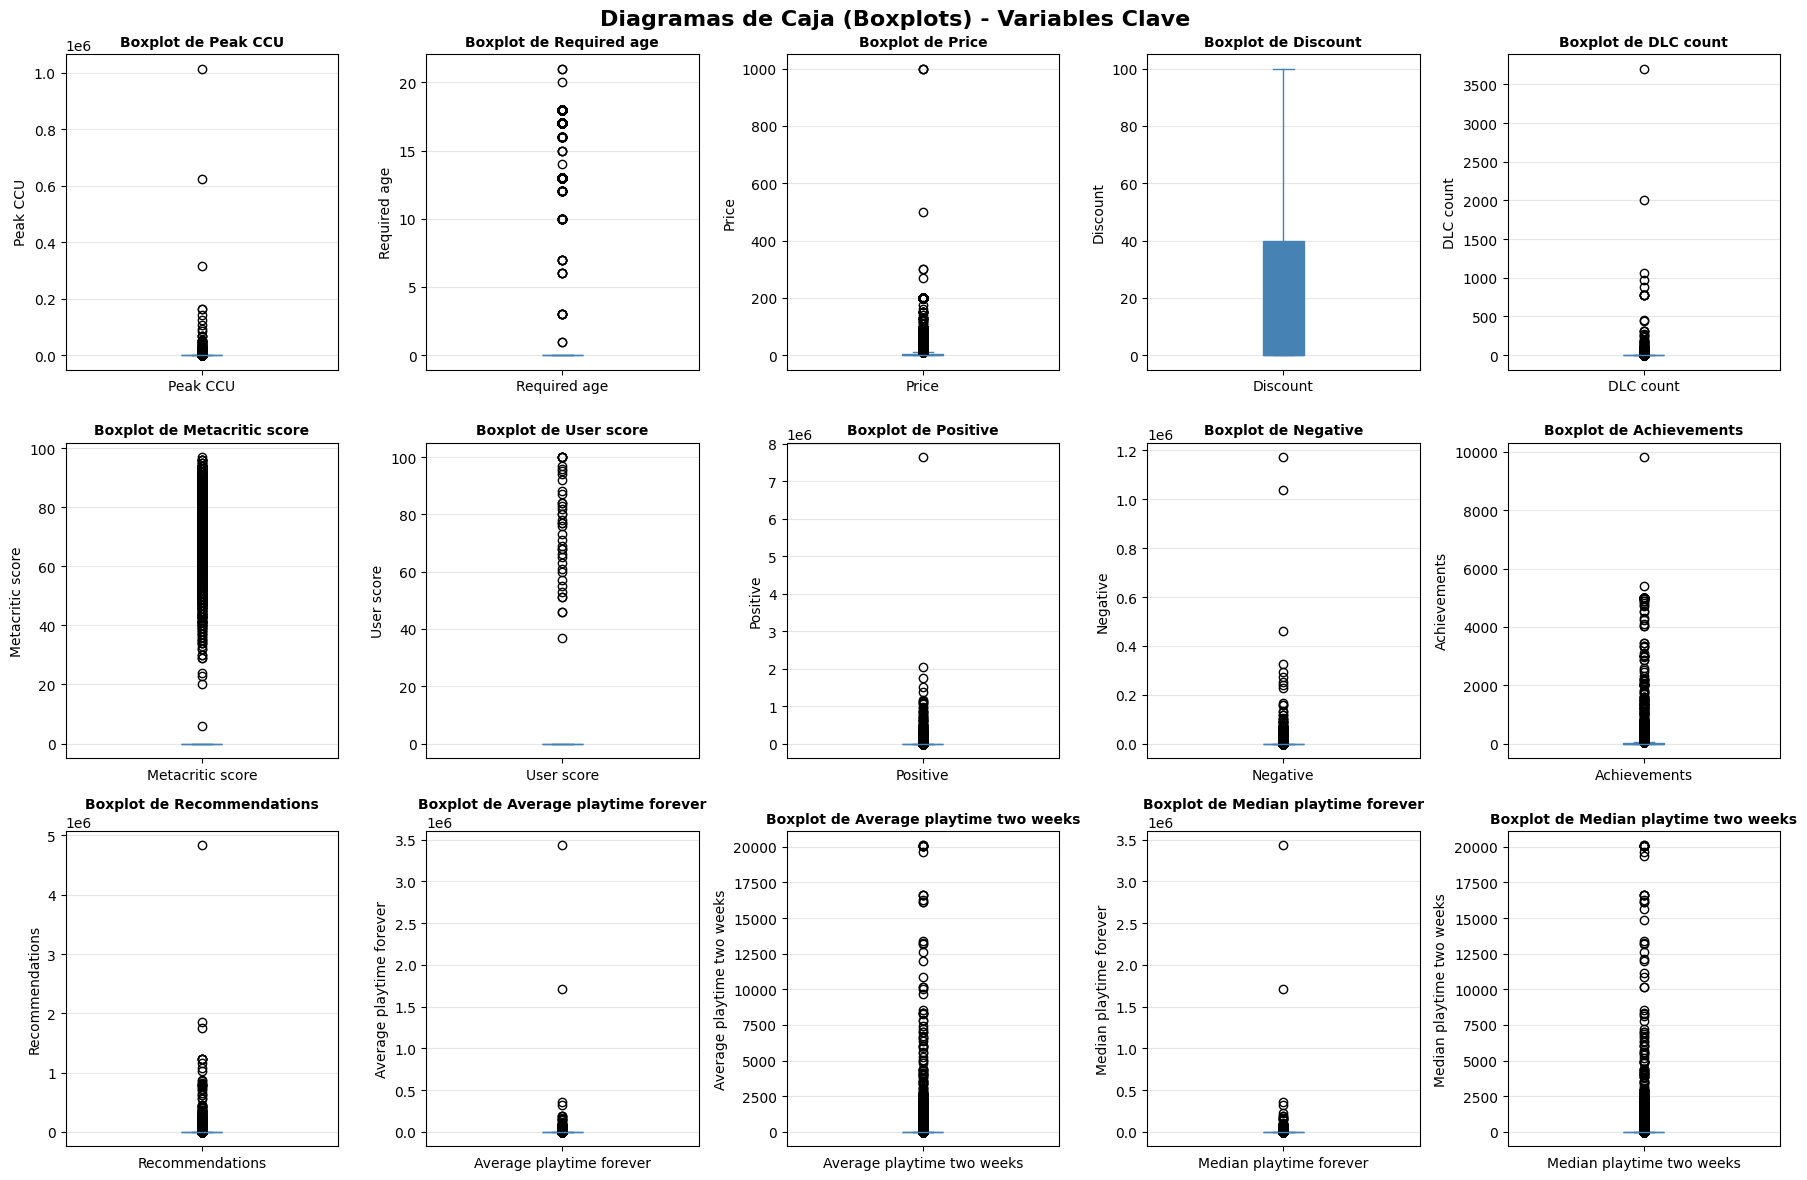
\includegraphics[width=\linewidth]{figures/grafica_5.png}}
  \caption{Diagramas de caja (\textit{Boxplots}) que muestran la gran cantidad de valores atípicos y la enorme dispersión generada por juegos sumamente populares.}
  \label{fig:boxplots}
\end{figure}

\subsection{Medidas de Dispersión y Distribuciones}
Para medir correctamente la dispersión de los datos sin afectar la precisión matemática a causa de de los valores atípicos, se priorizó la \textbf{Desviación Media Absoluta (AAD)}. Como se observa en la estimación de densidad KDE y en los diagramas de caja (Figura \ref{fig:boxplots}), atributos monetarios y de popularidad tienen una distribución marcadamente inclinada hacia la cota inferior. El mercado comercial se compone de innumerables títulos de bajo costo o completamente gratuitos con muy poco impacto, que contrastan fuertemente frente a las grandes y escasas franquicias \textit{AAA} o juegos virales.

\subsection{Causalidad Multivariada}
Al utilizar medidas de correlación lineal (coeficiente de Pearson), se encontraron relaciones claras y fundamentales. Por ejemplo, existe una fuerte asociación directa entre la máxima cifra récord de jugadores (\textit{Peak CCU}) y el volumen histórico de reseñas obtenidas (tanto positivas como negativas). Estos factores crecen directamente de acuerdo al volumen total de jugadores que atrae el título.

\section{Preprocesamiento de Datos}
Para asegurar que los datos del catálogo resulten óptimos para su uso en la fase de modelamiento algorítmico estadístico, se ejecutó un proceso riguroso de limpieza:

\subsection{Selección y Eliminación de Atributos}
Se descartaron todas las variables que no aportaban métricas relevantes para clasificar o predecir el éxito de un juego, tales como hipervínculos web, direcciones de correo de soporte y referencias multimedia promocionales (\textit{Header image}, \textit{Movies}, \textit{Screenshots}). Adicionalmente, se eliminaron columnas que se encontraban casi completamente vacías o rellenas de valores en cero, como \textit{User score} o \textit{Required age}, ya que estas interferían con la integridad de los modelos predictivos.

\begin{figure}[htbp]
  \centerline{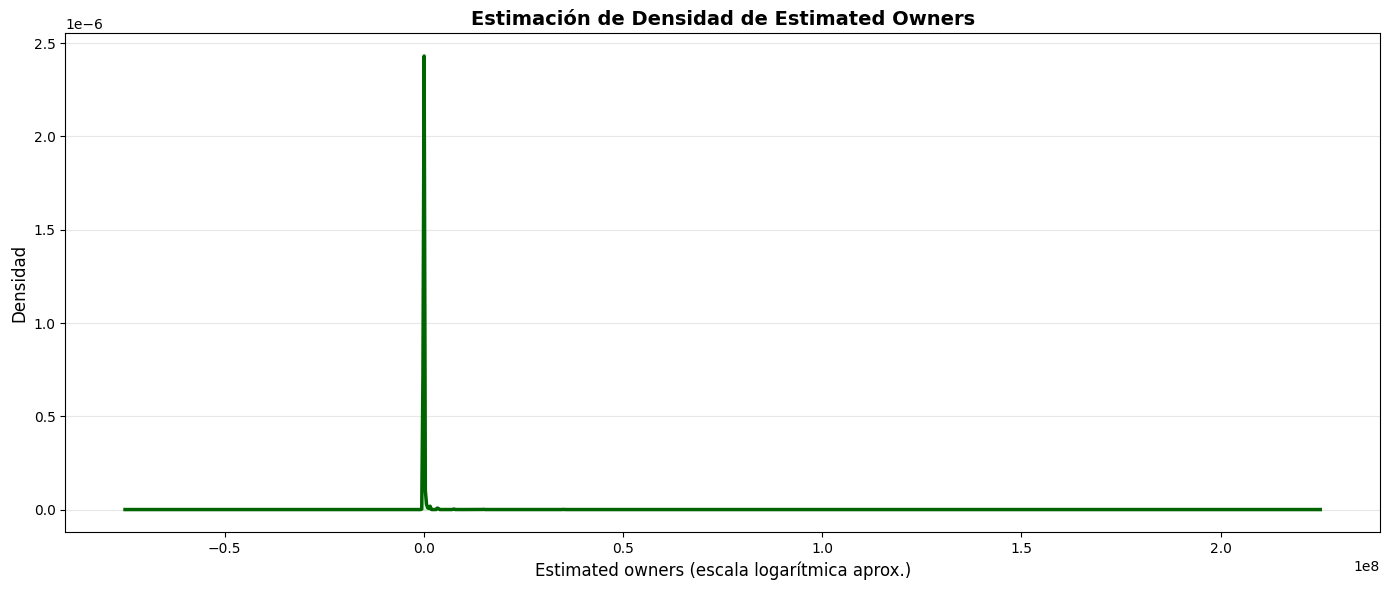
\includegraphics[width=\linewidth]{figures/grafica_4.png}}
  \caption{Estimación de densidad (KDE) para visibilizar las frecuencias en los rangos discretos de la cantidad estimada de jugadores (\textit{Estimated Owners}).}
  \label{fig:kde_owners}
\end{figure}

\subsection{Tratamiento de Valores Faltantes (Nulos)}
A través de la inspección sobre la ausencia de datos, se identificó que no figurar con un autor y empresa encargada (\textit{Developer}) es comúnmente una señal relacionada a estafas o desarrollos falsos subidos a la red de Steam; por este motivo, se purgaron completamente las filas que carecían de dicho identificador. Por el contrario, es un comportamiento normal que las variables categóricas o descriptivas queden en blanco (ej. \textit{Genres}, \textit{Tags}, \textit{Publishers}) debido a la forma de registro de algunos títulos. Estos casos orgánicos ausentes fueron cubiertos sistemáticamente con el identificador de texto ``NA'' para evitar corrupciones estructuradas. Toda métrica unívocamente matemática registró niveles completos, por lo que no existieron vacíos numéricos que imputar.

\subsection{Ingeniería de Atributos y Discretización}
El preprocesamiento del precio exhibía un desafío dada la enorme recurrencia de valores nominales fijados en \$0.00. Para contrarrestarlo, la cifra escalar \textit{Price} fue extraída bajo bandas de clasificación ordinales (\textit{Price\_category}), replicando las barreras comerciales comúnmente encontradas entre consumidores (juegos gratuitos, juegos muy baratos, o el tope tradicional de \$59.99). De igual forma lógica, la cadena textual correspondiente a la fecha de publicación (\textit{Release date}) se separó minuciosamente en tres diferentes campos tabulares: año, mes, y estación de lanzamiento. Esto habilitará la futura extracción estacional de picos de consumo anual.

\subsection{Manejo Condicional de Valores Atípicos}
La estrategia para atenuar valores atípicos se dictaminó con el algoritmo clásico del rango intercuartílico (IQR). En el campo preciso de los análisis tarifarios, se evidenció que aislar en dos sub-estratos independientes a los títulos ``Gratuitos'' en relación a aquellos de ``Pago'', provocaba un impacto determinante para comprender o fijar el límite estadístico a partir de cuándo un valor era realmente un costo sumamente atípico. Referente a medidas de popularidad de éxito irruptivo tales como la congregación máxima histórica (\textit{Peak CCU}), se optó intencionalmente por conservar intactos todos sus datos hiper-extendidos. Esto obedece a que limitar arbitrariamente dichos volúmenes resultaría en amputar a los protagonistas absolutos y al concepto fundamental del ``éxito'', mermando completamente las proyecciones algorítmicas hacia los verdaderos gigantes del mercado de videojuegos.

\subsection{Categorización de atributos}
Para facilitar el análisis de las reseñas, se crearon nuevas columnas con información derivada. Para empezar se crearon las columnas \texttt{total\_reviews} y \texttt{review\_rate}. La primera es el total de reseñas que tiene un juego, mientras que la segunda es la tase de reseñas positivas, calculada con la división entre las reseñas positivas (\textit{Positive}) y las reseñas totales. Con la tasa se realizó una categorización para manejar las reseñas, esta refleja la que se usa en la plataforma. Para empezar se analiza el número de reseñas, si son cero se asigna la categoría \textit{No reviews}, y si son menos de diez se tiene \textit{Too few reviews}. A partir de aquí, se toma la tasa para asignar las categorías además del número de reseñas.

\begin{table}[]
\begin{tabular}{lll}
Categorías              & Reseñas mínimas & Tasa mínima \\
Overwhelmingly Positive & 500             & 0,95        \\
Very Positive           & 10              & 0,8         \\
Mostly Positive         & 10              & 0,7         \\
Mixed                   & 10              & 0,4         \\
Mostly Negative         & 10              & 0,2         \\
Overwhelmingly Negative & 500             & 0,2         \\
Very Negative           & 50              & 0,2        
\end{tabular}
\end{table}

También se creó una categorización para las ventas, con el atributo "No data" para aquellos juegos sin ventas. A partir de aquí se tienen las siguientes categorías:

\begin{table}[]
\begin{tabular}{ll}
Categorías        & Ventas Máximas   \\
Niche             & 20000            \\
Small Indie       & 100000           \\
Growing           & 500000           \\
Popular           & 1000000          \\
Very Popular      & 2000000          \\
Top Game          & 10000000         \\
Blockbuster       & 50000000        
\end{tabular}
\end{table}

Adicionalmente, se tiene la categoría "Mega Hit" para los juegos que tengan más de 50000000 de ventas.

Por último, también se tiene una categorización de desempeño con base en las métricas del pico de usuarios concurrentes ("Peak CCU") y la calificación de la página agregadora de reseñas Metacritic.

Para los usuarios concurrentes se realiza una clasificación por percentiles con los valores de 0.25, 0.5, 0.75 y 0.9. Estos definen las categorías, los juegos con un valor de 0 son asignados a la categoría "No activity", mientras que los demás se asignan a las categorías "Very Low", "Low", "Medium" y "High". Los juegos en el percentil más alto entran en la categoría "Very High".

Respecto a la calificación de Metacritic, la clasificación se hace teniendo en cuenta ciertos sesgos de la plataforma, donde la calificación de muchos juegos tiende a estar entre 50 y 100, y rara vez se otorga una clasificación menor a 50. Con esto en mente se tienen las categorías "Not rated" para juegos sin calificación, "Poor" para aquellos con menos de 50, "Mediocre" hasta 60, "Average" hasta 70, "Good" hasta 80, "Very Good" hasta 90 y "Excellent" para los juegos con una calificación entre 91 y 100.

\subsection{Juegos de interés}
Para analizar distintas tendencias se hizo una selección separada de ciertos juegos particularmente exitosos, estos fueron denominados como juegos de interés. Para seleccionar estos juegos se decidieron las medidas de reseñas y ventas, selecionando los juegos con reseñas de Steam en las categorías Overwhelmingly Positive o Very Positive, o ventas en las categorías Top Game, Blockbuster o Mega Hit.

\subsection{Uso de One-Hot Encoding}
Se realizó el One-Hot Encoding en los atributos de "Genres" y "Tags" para facilitar el análisis. Sobre los géneros se realizó la codifiación sobre los 33 géneros únicos del dataset, mientras que para las etiquetas solo se usaron aquellas que tengan al menos 5000 apariciones para evitar tener columnas demasiado dispersas, conservando 59 de las 452 etiquetas presentes en el dataset.

\section{Análisis de reglas de asociación}
En esta sección se aplicaron los algoritmos Apriori y FP-Growth para generar reglas de asociación con base en los géneros y las etiquetas. Para empezar se realizó el análsis del dataset completo usando ciertas caracterísitcas de los juegos como antecedentes y métricas de éxito como consecuentes. Posteriormente se pasó al análisis de los juegos de interés, generando reglas de asociación entre géneros y etiquetas para obtener información específica a estos juegos. Por último se analizaron los juegos de interés para obtener las características que conducen a una calificación extremadamente positiva entre estos juegos.

\subsection{Análisis del dataset completo}
Para el análisis del dataset completo se usaron como antecedentes las columans que se consideraron útiles para predecir el éxito de un juego: \texttt{genre} y \texttt{tag} definen el contenido y estilo del juego, \texttt{Categories} da los modos de juego disponibles, \texttt{Price\_category} defiene el precio del juego, \texttt{Release\_season} y \texttt{Release\_year} hablan del contexto del mercado, \texttt{Windows}, \texttt{Mac}, \texttt{Linux} dan el alcance de la plataforma y, por último, \texttt{DLC\_count} y \texttt{Discount} se toman en bins y dan los contenidos descargables disponibles y los descuentos aplicados a los precios.

Respecto a los consecuentes, se seleccionaron como medidas de éxito la calificación de los juegos (\texttt{review\_score\_cat}) con el objetivo de reseñas favorables, el volumen de reseñas (\texttt{total\_reviews}) con los objetivos de reseñas por encima del percentil 50, las ventas (\texttt{sales\_cat}) con el objetivo \texttt{sales\_good} y el pico de usuarios concurrentes (\texttt{ccu\_cat}) con el objetivo \texttt{ccu\_good}.

Durante la aplicación de los algoritmos se pusieron restricciones a los soportes mínimo y máximo para descartar items raros y descartar tiems demasiado comunes (poco informativos).

Las tablas muestran las 10 mejores reglas generadas por los dos algoritmos para cada consecuente, seguido de las 10 reglas globales más frecuentes. 

\begin{table}[]
\resizebox{\columnwidth}{!}{%
\begin{tabular}{rrrrrr}
\textbf{} & \textbf{antecedents}                      & \textbf{consequents} & \textbf{support} & \textbf{confidence} & \textbf{lift} \\
1         & cat=Steam Trading Cards, tag=2D           & target=review\_good  & 0.023683         & 0.836116            & 2.361186      \\
2         & DLC=1-2, tag=Story Rich                   & target=review\_good  & 0.022834         & 0.807371            & 2.280008      \\
3         & cat=Steam Cloud, tag=Anime                & target=review\_good  & 0.024086         & 0.801749            & 2.264134      \\
4         & cat=Steam Trading Cards, tag=Singleplayer & target=review\_good  & 0.043635         & 0.797248            & 2.251421      \\
5         & cat=Steam Cloud, tag=Story Rich           & target=review\_good  & 0.034868         & 0.793186            & 2.239951      \\
6         & DLC=1-2, tag=Atmospheric                  & target=review\_good  & 0.020880         & 0.791764            & 2.235934      \\
7         & cat=Steam Cloud, tag=Female Protagonist   & target=review\_good  & 0.021240         & 0.785298            & 2.217675      \\
8         & DLC=1-2, tag=2D                           & target=review\_good  & 0.030226         & 0.773247            & 2.183643      \\
9         & cat=Steam Cloud, tag=Funny                & target=review\_good  & 0.023578         & 0.772675            & 2.182028      \\
10        & cat=Steam Cloud, cat=Steam Trading Cards  & target=review\_good  & 0.043539         & 0.765476            & 2.161698     
\end{tabular}%
}
\label{target review good fp growth 126 total rules}
\end{table}

\begin{table}[]
\resizebox{\columnwidth}{!}{%
\begin{tabular}{rrrrrr}
\textbf{} & \textbf{antecedents}    & \textbf{consequents} & \textbf{support} & \textbf{confidence} & \textbf{lift} \\
1         & tag=Visual Novel        & target=review\_good  & 0.034360         & 0.673708            & 1.902545      \\
2         & cat=Steam Trading Cards & target=review\_good  & 0.066933         & 0.673245            & 1.901238      \\
3         & tag=Anime               & target=review\_good  & 0.047331         & 0.662174            & 1.869973      \\
4         & tag=Difficult           & target=review\_good  & 0.035814         & 0.644140            & 1.819046      \\
5         & tag=Story Rich          & target=review\_good  & 0.074404         & 0.636616            & 1.797798      \\
6         & tag=Female Protagonist  & target=review\_good  & 0.041945         & 0.631878            & 1.784417      \\
7         & tag=Comedy              & target=review\_good  & 0.032932         & 0.629289            & 1.777106      \\
8         & tag=Multiple Endings    & target=review\_good  & 0.028746         & 0.614032            & 1.734021      \\
9         & tag=Funny               & target=review\_good  & 0.053007         & 0.613855            & 1.733523      \\
10        & tag=Cute                & target=review\_good  & 0.066635         & 0.600047            & 1.694529     
\end{tabular}%
}
\label{target review good apriori 37 total rules}
\end{table}

\begin{table}[]
\resizebox{\columnwidth}{!}{%
\begin{tabular}{rrrrrr}
\textbf{} & \textbf{antecedents}    & \textbf{consequents} & \textbf{support} & \textbf{confidence} & \textbf{lift} \\
1         & tag=Co-op               & target=sales\_good   & 0.007769         & 0.168695            & 7.679673      \\
2         & tag=Multiplayer         & target=sales\_good   & 0.012297         & 0.138407            & 6.300827      \\
3         & tag=Open World          & target=sales\_good   & 0.007191         & 0.137016            & 6.237507      \\
4         & cat=Steam Trading Cards & target=sales\_good   & 0.011544         & 0.116113            & 5.285925     
\end{tabular}%
}
\label{target sales good fp growth apriori 4 total rules}
\end{table}

\begin{table}[]
\resizebox{\columnwidth}{!}{%
\begin{tabular}{rrrrrr}
\textbf{} & \textbf{antecedents}    & \textbf{consequents} & \textbf{support} & \textbf{confidence} & \textbf{lift} \\
1         & tag=Multiplayer         & target=ccu\_good     & 0.017298         & 0.194696            & 4.605192      \\
2         & cat=Steam Trading Cards & target=ccu\_good     & 0.016624         & 0.167210            & 3.955050      \\
3         & cat=Co-op               & target=ccu\_good     & 0.011412         & 0.118401            & 2.800556      \\
4         & cat=Multi-player        & target=ccu\_good     & 0.017902         & 0.100839            & 2.385157      \\
5         & DLC=1-2                 & target=ccu\_good     & 0.012402         & 0.100276            & 2.371853     
\end{tabular}%
}
\label{target ccu good fp growth apriori 5 total rules}
\end{table}

\begin{table}[]
\resizebox{\columnwidth}{!}{%
\begin{tabular}{rllrrr}
\textbf{} & \textbf{antecedents}                            & \textbf{consequents}      & \textbf{support} & \textbf{confidence} & \textbf{lift} \\
1         & cat=Steam Trading Cards, tag=Story Rich         & target=reviews\_50p\_plus & 0.021853         & 0.998000            & 1.955074      \\
2         & cat=Steam Trading Cards, tag=Atmospheric        & target=reviews\_50p\_plus & 0.021975         & 0.996822            & 1.952766      \\
3         & cat=Steam Trading Cards, tag=RPG                & target=reviews\_50p\_plus & 0.023053         & 0.992459            & 1.944219      \\
4         & cat=Steam Trading Cards, tag=Adventure          & target=reviews\_50p\_plus & 0.046184         & 0.991725            & 1.942781      \\
5         & cat=Steam Trading Cards, tag=Strategy           & target=reviews\_50p\_plus & 0.022982         & 0.991686            & 1.942705      \\
6         & cat=Steam Trading Cards, tag=Action             & target=reviews\_50p\_plus & 0.045860         & 0.987179            & 1.933877      \\
7         & cat=Steam Trading Cards, tag=Indie              & target=reviews\_50p\_plus & 0.061800         & 0.985613            & 1.930808      \\
8         & Release\_era=2010-2019, cat=Steam Trading Cards & target=reviews\_50p\_plus & 0.069315         & 0.979819            & 1.919459      \\
9         & Release\_era=2010-2019, tag=Female Protagonist  & target=reviews\_50p\_plus & 0.020162         & 0.962375            & 1.885285      \\
10        & Discount=51-75, cat=Steam Trading Cards         & target=reviews\_50p\_plus & 0.021485         & 0.961584            & 1.883735     
\end{tabular}%
}
\label{target reviews 50p fp growth 192 total rules}
\end{table}

\begin{table}[]
\resizebox{\columnwidth}{!}{%
\begin{tabular}{rllrrr}
\textbf{} & \textbf{antecedents}     & \textbf{consequents}      & \textbf{support} & \textbf{confidence} & \textbf{lift} \\
1         & cat=Steam Trading Cards  & target=reviews\_50p\_plus & 0.092508         & 0.930491            & 1.822824      \\
2         & tag=Co-op                & target=reviews\_50p\_plus & 0.038249         & 0.830544            & 1.627029      \\
3         & tag=Anime                & target=reviews\_50p\_plus & 0.059252         & 0.828943            & 1.623892      \\
4         & tag=Difficult            & target=reviews\_50p\_plus & 0.045466         & 0.817738            & 1.601942      \\
5         & Discount=76+             & target=reviews\_50p\_plus & 0.058971         & 0.813262            & 1.593175      \\
6         & tag=Visual Novel         & target=reviews\_50p\_plus & 0.041270         & 0.809205            & 1.585226      \\
7         & tag=Multiplayer          & target=reviews\_50p\_plus & 0.071785         & 0.807965            & 1.582798      \\
8         & tag=Psychological Horror & target=reviews\_50p\_plus & 0.042996         & 0.804754            & 1.576507      \\
9         & Release\_era=2010-2019   & target=reviews\_50p\_plus & 0.211248         & 0.803859            & 1.574755      \\
10        & tag=Female Protagonist   & target=reviews\_50p\_plus & 0.053138         & 0.800501            & 1.568176     
\end{tabular}%
}
\label{target reviews 50p apriori 37 total rules}
\end{table}

\begin{table}[]
\resizebox{\columnwidth}{!}{%
\begin{tabular}{rllrrr}
\textbf{} & \textbf{antecedents}                            & \textbf{consequents}      & \textbf{support} & \textbf{confidence} & \textbf{lift} \\
1         & cat=Steam Trading Cards, tag=Atmospheric        & target=reviews\_75p\_plus & 0.020872         & 0.946762            & 3.783138      \\
2         & cat=Steam Trading Cards, tag=Story Rich         & target=reviews\_75p\_plus & 0.020626         & 0.942000            & 3.764110      \\
3         & cat=Steam Trading Cards, tag=RPG                & target=reviews\_75p\_plus & 0.020819         & 0.896305            & 3.581517      \\
4         & cat=Steam Trading Cards, tag=Adventure          & target=reviews\_75p\_plus & 0.040613         & 0.872108            & 3.484832      \\
5         & cat=Steam Trading Cards, tag=Strategy           & target=reviews\_75p\_plus & 0.020153         & 0.869615            & 3.474867      \\
6         & DLC=1-2, cat=Steam Trading Cards                & target=reviews\_75p\_plus & 0.026565         & 0.859938            & 3.436199      \\
7         & Release\_era=2010-2019, tag=Multiplayer         & target=reviews\_75p\_plus & 0.025277         & 0.842628            & 3.367031      \\
8         & cat=Steam Cloud, cat=Steam Trading Cards        & target=reviews\_75p\_plus & 0.047822         & 0.840776            & 3.359632      \\
9         & cat=Steam Trading Cards, platform=Mac           & target=reviews\_75p\_plus & 0.030602         & 0.824445            & 3.294377      \\
10        & Release\_era=2010-2019, cat=Steam Trading Cards & target=reviews\_75p\_plus & 0.056983         & 0.805497            & 3.218662     
\end{tabular}%
}
\label{target reviews 75p fp growth 87 total rules}
\end{table}

\begin{table}[]
\resizebox{\columnwidth}{!}{%
\begin{tabular}{rllrrr}
\textbf{} & \textbf{antecedents}    & \textbf{consequents}      & \textbf{support} & \textbf{confidence} & \textbf{lift} \\
1         & cat=Steam Trading Cards & target=reviews\_75p\_plus & 0.079020         & 0.794820            & 3.175997      \\
2         & tag=Co-op               & target=reviews\_75p\_plus & 0.027038         & 0.587105            & 2.345997      \\
3         & tag=Multiplayer         & target=reviews\_75p\_plus & 0.051089         & 0.575020            & 2.297704      \\
4         & tag=Anime               & target=reviews\_75p\_plus & 0.038555         & 0.539395            & 2.155351      \\
5         & tag=Open World          & target=reviews\_75p\_plus & 0.028027         & 0.534045            & 2.133976      \\
6         & DLC=1-2                 & target=reviews\_75p\_plus & 0.063193         & 0.510941            & 2.041655      \\
7         & Discount=76+            & target=reviews\_75p\_plus & 0.036777         & 0.507187            & 2.026653      \\
8         & tag=Female Protagonist  & target=reviews\_75p\_plus & 0.033414         & 0.503365            & 2.011379      \\
9         & tag=Story Rich          & target=reviews\_75p\_plus & 0.057798         & 0.494529            & 1.976075      \\
10        & Release\_era=2010-2019  & target=reviews\_75p\_plus & 0.122497         & 0.466138            & 1.862626     
\end{tabular}%
}
\label{target reviews 75p apriori 34 total rules}
\end{table}

\begin{table}[]
\resizebox{\columnwidth}{!}{%
\begin{tabular}{rrrrrr}
\textbf{} & \textbf{antecedents}                     & \textbf{consequents}      & \textbf{support} & \textbf{confidence} & \textbf{lift} \\
1         & tag=Co-op                                & target=sales\_good        & 0.007769         & 0.168695            & 7.679673      \\
2         & tag=Multiplayer                          & target=sales\_good        & 0.012297         & 0.138407            & 6.300827      \\
3         & tag=Open World                           & target=sales\_good        & 0.007191         & 0.137016            & 6.237507      \\
4         & cat=Steam Trading Cards                  & target=sales\_good        & 0.011544         & 0.116113            & 5.285925      \\
5         & tag=Multiplayer                          & target=ccu\_good          & 0.017298         & 0.194696            & 4.605192      \\
6         & cat=Steam Trading Cards                  & target=ccu\_good          & 0.016624         & 0.167210            & 3.955050      \\
7         & cat=Steam Trading Cards, tag=Atmospheric & target=reviews\_75p\_plus & 0.020872         & 0.946762            & 3.783138      \\
8         & cat=Steam Trading Cards, tag=Story Rich  & target=reviews\_75p\_plus & 0.020626         & 0.942000            & 3.764110      \\
9         & cat=Steam Trading Cards, tag=RPG         & target=reviews\_75p\_plus & 0.020819         & 0.896305            & 3.581517      \\
10        & cat=Steam Trading Cards, tag=Adventure   & target=reviews\_75p\_plus & 0.040613         & 0.872108            & 3.484832     
\end{tabular}%
}
\label{top 10 global fp-growth}
\end{table}

\begin{table}[]
\resizebox{\columnwidth}{!}{%
\begin{tabular}{rllrrr}
\textbf{} & \textbf{antecedents}    & \textbf{consequents}      & \textbf{support} & \textbf{confidence} & \textbf{lift} \\
1         & tag=Co-op               & target=sales\_good        & 0.007769         & 0.168695            & 7.679673      \\
2         & tag=Multiplayer         & target=sales\_good        & 0.012297         & 0.138407            & 6.300827      \\
3         & tag=Open World          & target=sales\_good        & 0.007191         & 0.137016            & 6.237507      \\
4         & cat=Steam Trading Cards & target=sales\_good        & 0.011544         & 0.116113            & 5.285925      \\
5         & tag=Multiplayer         & target=ccu\_good          & 0.017298         & 0.194696            & 4.605192      \\
6         & cat=Steam Trading Cards & target=ccu\_good          & 0.016624         & 0.167210            & 3.955050      \\
7         & cat=Steam Trading Cards & target=reviews\_75p\_plus & 0.079020         & 0.794820            & 3.175997      \\
8         & cat=Co-op               & target=ccu\_good          & 0.011412         & 0.118401            & 2.800556      \\
9         & cat=Multi-player        & target=ccu\_good          & 0.017902         & 0.100839            & 2.385157      \\
10        & DLC=1-2                 & target=ccu\_good          & 0.012402         & 0.100276            & 2.371853     
\end{tabular}%
}
\label{top 10 global apriori}
\end{table}

\subsection{Análisis de los juegos de interés}

\begin{figure}[htbp]
  \centerline{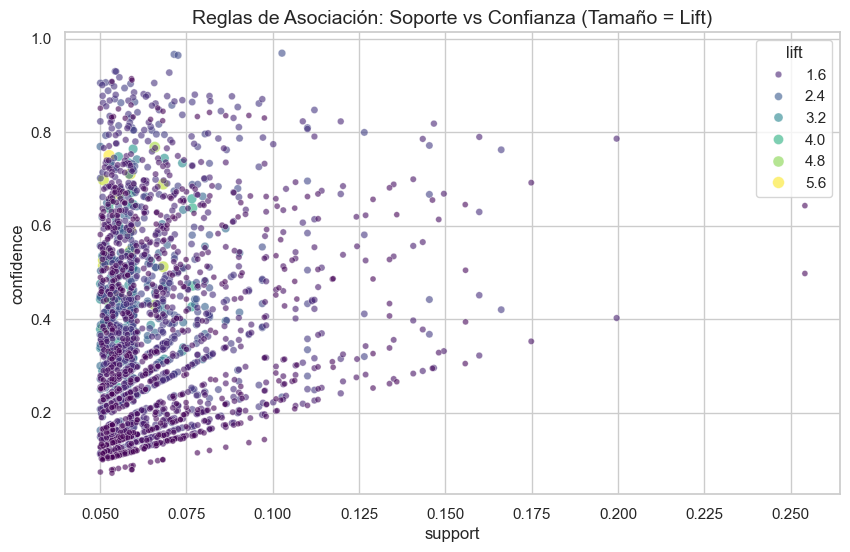
\includegraphics[width=\linewidth]{figures/grafica_7.png}}
  \caption{Reglas de asociación de los juegos de interés.}
  \label{fig:as_rules1}
\end{figure}

\begin{figure}[htbp]
  \centerline{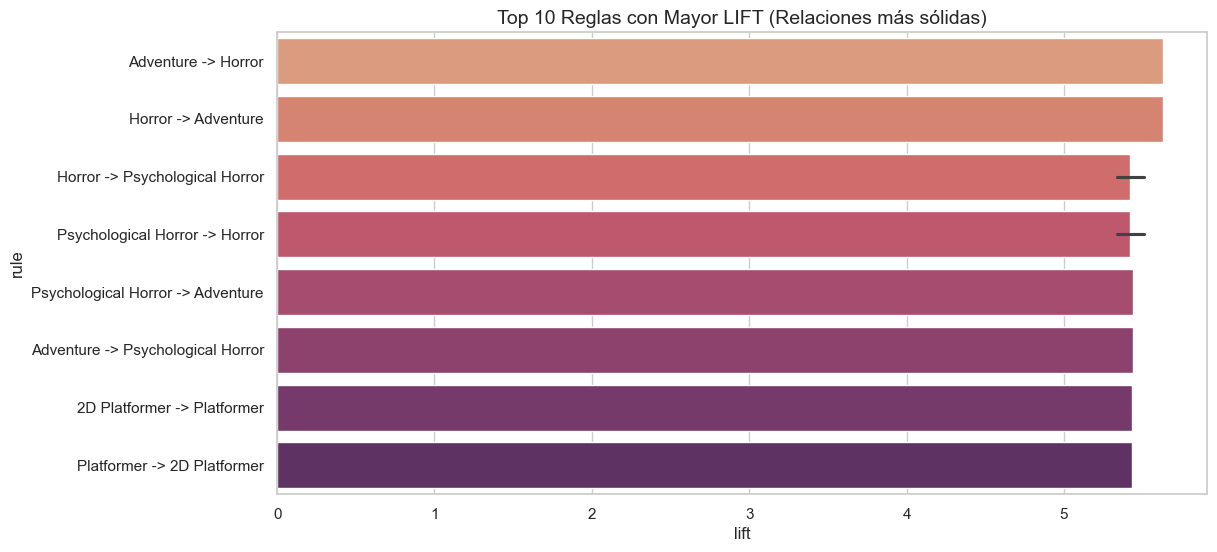
\includegraphics[width=\linewidth]{figures/grafica_8.png}}
  \caption{Reglas con mayor lift en el primer análsis.}
  \label{fig:as_rules_top10_1}
\end{figure}

En los juegos de interés se utilizó el algoritmo Apriori para encontrar las relaciones entre géneros para encontrar las combinaciones más frecuentes. Con este algoritmo se encontraron 2288 regals de asociación, ilustradas con su soporte y confianza en la figura \ref{fig:as_rules1}. Las 10 reglas con mayor lift se ilustran en la figura \ref{fig:as_rules_top10_1}.

Sin embargo, muchas de las reglas descubiertas con este método corresponden a jerarquías naturales de clasificación, como es el caso de la regla \texttt{Psychological Horror -> Horror}, o conceptos sumamente amplios. Por esto se aplicaron dos estrategias de filtrado avanzado: la primera es la exclusión de etiquetas genéricas ("Stop-Tags"), donde se retiran ciertas etiquetas que no aportan diferenciación. La segunda es el análisis de reglas complejas, donde se buscan reglas con al menos 3 elementos para obtener información más valiosa.

\begin{figure}[htbp]
  \centerline{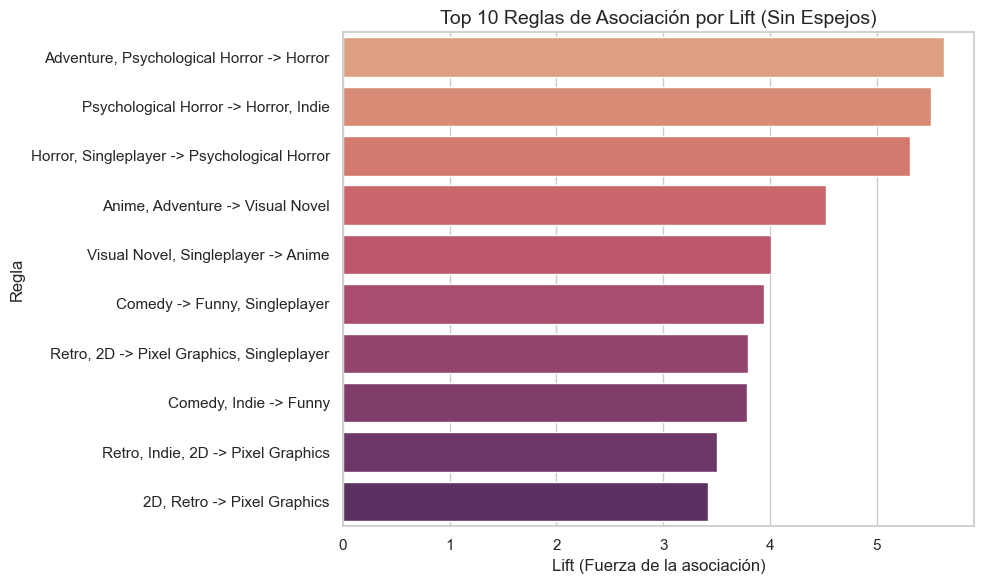
\includegraphics[width=\linewidth]{figures/grafica_9.png}}
  \caption{Reglas con mayor lift en el análsis con las dos estrategias aplicadas.}
  \label{fig:as_rules_top10_2}
\end{figure}

Al aplicar estas dos estrategias, se obtuvieron 2060 reglas, de las cuales las 10 con mayor lift se encuentran en la figura \ref{fig:as_rules_top10_2}.

\begin{figure}[htbp]
  \centerline{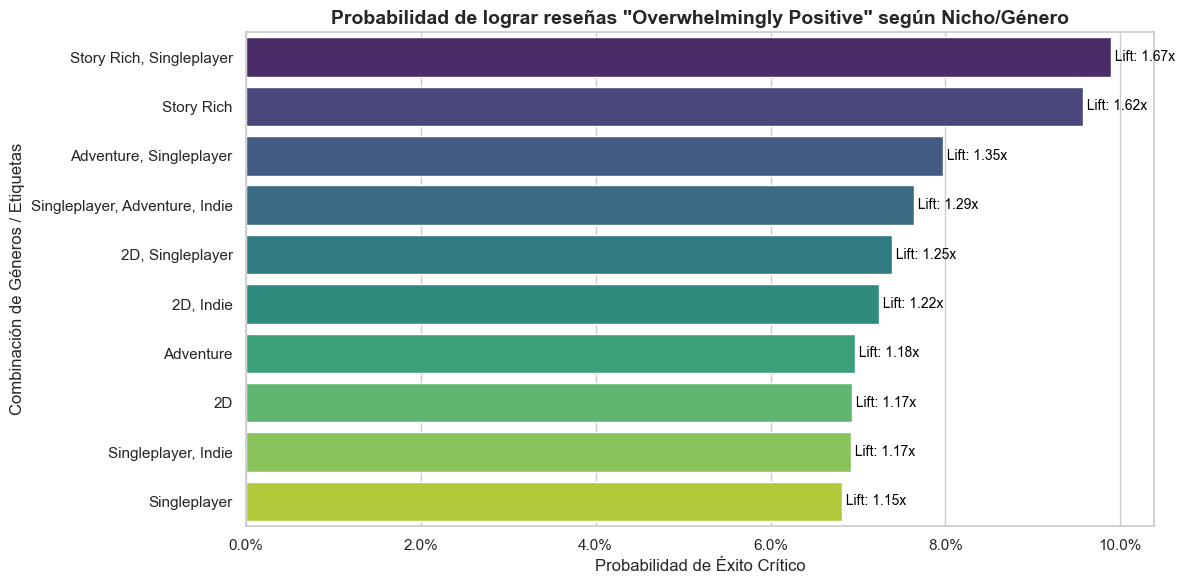
\includegraphics[width=\linewidth]{figures/grafica_10.png}}
  \caption{Reglas con mayor lift en el análsis con las dos estrategias aplicadas.}
  \label{fig:as_rules_top10_3}
\end{figure}

A continuación, se realizó el análisis de los juegos de interés orientado a la creación de reglas con el consecuente "Overwhelmingly Positive" en la variable \texttt{review\_score\_cat}. Las 10 combinaciones que tienen este consecuente se muestran en la figura \ref{fig:as_rules_top10_3}.

Por último, se realizó la ejecución del algoritmo FP-Growth sobre los mismos datos, obteniendo resultados idénticos en las reglas pero con una mejora notable en el desempeño del algoritmo, obteniendo el mismo número de itemsets 4.7 veces más rápidamente.

\section{Análisis de la agrupación}
Para realizar un análisis de los juegos según su rendimiento se realizó el agrupamiento de los juegos de interés. Este tipo de análisis también se intentó con el dataset completo. Sin embargo, debido a la cantidad de datos, los análisis intentados no se pudieron completar.

\subsection{Análsis del dataset completo}
Para la agrupación se seleccionaron como variables el porcentaje de reseñas positivas (\texttt{Positive}), el número de compradores estimado (\texttt{Estimated owners}) y el pico de jugadores concurrentes (\texttt{Peak CCU}). Se eliminaron las filas con valores nulos en estas variables y se normalizaron.

\begin{figure}[htbp]
  \centerline{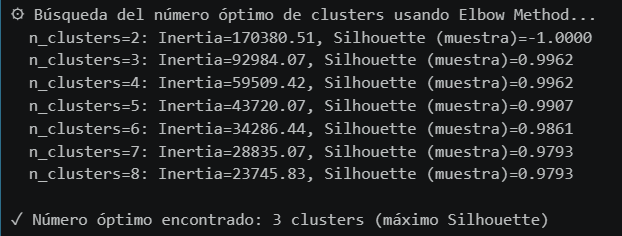
\includegraphics[width=\linewidth]{figures/grafica_11.png}}
  \caption{Valores generados con cada n usando el algoritmo K-Means.}
  \label{fig:ag_dc_elbow}
\end{figure}


Se utilizó primero el algoritmo K-Means con distintas cantidades de clusters, esto con el objetivo de encontrar el valor que maximizara el Silhouette, el cual fue de 3 clusters. Los resultados se muestran en la figura \ref{fig:ag_dc_elbow}.

\begin{figure}[htbp]
  \centerline{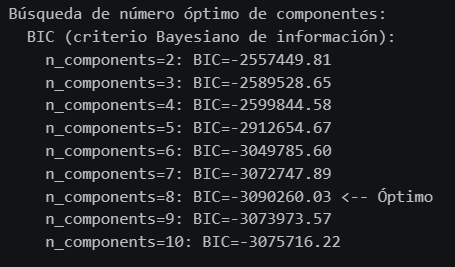
\includegraphics[width=\linewidth]{figures/grafica_12.png}}
  \caption{Valores generados con cada n en el algoritmo GMM.}
  \label{fig:ag_dc_elbow_2}
\end{figure}

Para la segunda prueba se utilizó el algoritmo GMM (Gaussian Mixture Model). En este se utilizó el criterio Bayesiano de información para obtener el número óptimo de n, el cuál fue de 8. Esto se evidencia en la figura \ref{fig:ag_dc_elbow_2}.

A pesar de que los dos algoritmos se ejecutaron exitosamente, no fue posible obtener más información de los clusters debido a que no se puedo ejecutar el código para la comparación y la graficación en tres dimensiones.

\subsection{Análisis de los juegos de interés}

\begin{figure}[htbp]
  \centerline{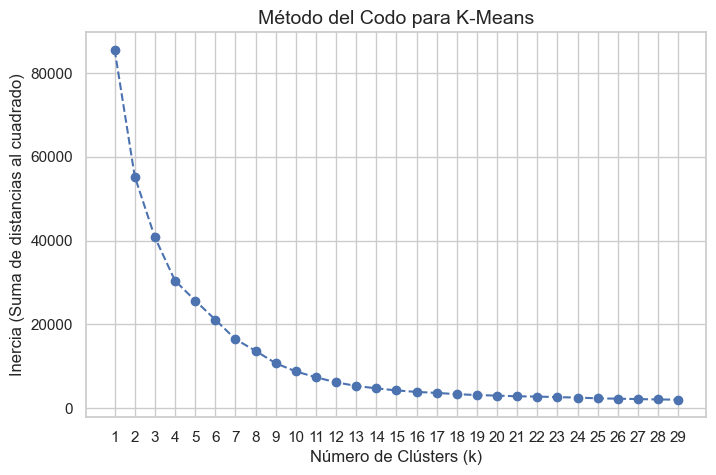
\includegraphics[width=\linewidth]{figures/grafica_13.png}}
  \caption{Gráfica de codo generada para los juegos de interés con el algoritmo K-Means.}
  \label{fig:ag_ji_elbow}
\end{figure}

En el caso de los juegos de interés se empleó primero el algoritmo K-means sobre cuatro variables que definen el perfil comercial del juego: El precio (\texttt{Price}), pico de usuarios concurrentes \texttt{Peak CCU}, porcentaje de reseñas positivas (\texttt{Positive}) y promedio de timepo jugado \texttt{Average playtime forever}. De manera similar al análisis de los datos en genral primero se normalizaron los datos y más adelante se usó el método del codo para encontrar el número óptimo de clusters. Este método se encuentra graficado en la figura \ref{fig:ag_ji_elbow}.

\begin{figure}[htbp]
  \centerline{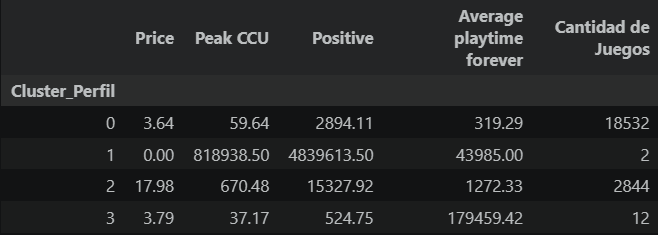
\includegraphics[width=\linewidth]{figures/tabla_1.png}}
  \caption{Tabla generada con los promedios de las variables en cada cluster.}
  \label{fig:ag_ji_table}
\end{figure}

Se tomó el valor n como cuatro, y los valores promedio de cada cluster se encuentran en la figura \ref{fig:ag_ji_table}.

Con estas métricas se puede hacer un análisis de cada cluster para comprender los perfiles comerciales de los juegos exitosos.

\begin{itemize}
  \item Éxito general: El cluster más grande tiene precios accesibles y tiempos de juego cercanos al promedio.
  \item Juegos premium: En este grupo los juegos tienen un valor más elevado, con grandes cantidades de reseñas positivas y altos picos de jugadores.
  \item Juegos Idle: Unos pocos juegos con bajos precios, reseñas y jugadores, pero con una cantidad muy alta de tiempo de juego. Estos juegos son aquellos que se pueden dejar corriendo de fondo mientras los usuarios hacen otras tareas.
  \item Duopolio Free-to-play: El último cluster lo componen solo dos juegos: Counter-Strike 2 y Dota 2. Estos dos juegos son gratuitos, con una gran cantidad de usuarios y tiempo de juego. Se podría considerar que estos juegos tienen un ecosistema económico independiente.
\end{itemize}

\begin{figure}[htbp]
  \centerline{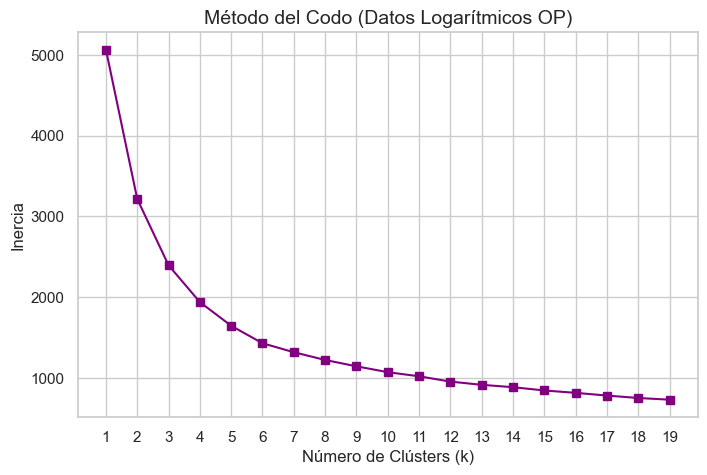
\includegraphics[width=\linewidth]{figures/grafica_14.png}}
  \caption{Gráfica de codo del algoritmo K-Means en los juegos con reseñas muy positivas con los datos con transformación logarítmica.}
  \label{fig:ag_ji_log_elbow}
\end{figure}

Para robustecer el análisis del algoritmo K-Means se aplica una transformación logarítmica a los datos para reducir el impacto de juegos con métricas extremas y se busca comprender la razón por la que ciertos juegos tienen la calificación \texttt{Overwhelmingly Positive}. El análisis genera la gráfica de codo de la figura \ref{fig:ag_ji_log_elbow}.

\begin{figure}[htbp]
  \centerline{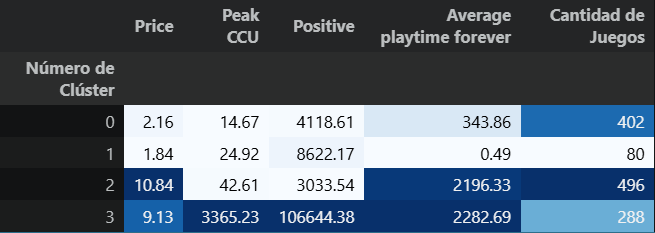
\includegraphics[width=\linewidth]{figures/tabla_2.png}}
  \caption{Clusters generados por el algoritmo K-Means usando datos con transformación logarítmica.}
  \label{fig:ag_ji_log_table}
\end{figure}

Con esta ejecución del algoritmo se encontraron los clusters de la figura \ref{fig:ag_ji_log_table}.

Con los dos análisis se encontraron dos grandes divisiones:

\begin{itemize}
  \item Entre los juegos de precio medio/alto se encontraron dos grupos con buenas retenciones de juego, pero diferenciados por la popularidad, representada en el pico de usuarios concurrentes. Por un lado se tienen juegos muy conocidos con un CCU muy elevado, y por otro juegos aclamados pero menos populares, con buena retención pero un bajo pico de usuarios concurrentes.
  \item  Entre los juegos gratuitos o de bajo costo se tiene una división basada en el tiempo de juego promedio, con una división entre los juegos con un tiempo de juego razonable y aquellos con muy poco tiempo, catalogados como herramientas o registros erróneos.
\end{itemize}

\begin{figure}[htbp]
  \centerline{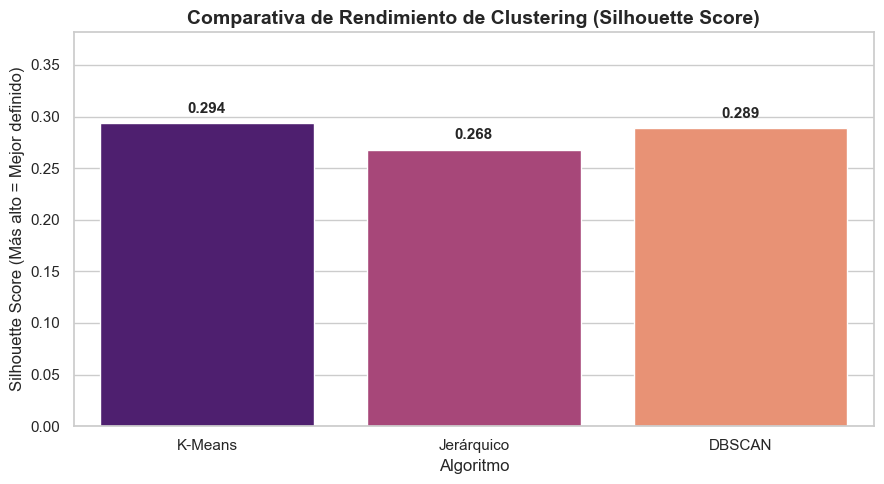
\includegraphics[width=\linewidth]{figures/grafica_15.png}}
  \caption{Rendimiento de los algortimos evaluados con base en el coeficiente de Silueta.}
  \label{fig:ag_ji_sil}
\end{figure}

Para realizar una comparación, se utilizaron otros dos algoritmos para realizar una comparativa entre las tres grandes familias de clustering no supervisado. Como K-Means es un algoritmo particional, su utilizó Agglomerative Clustering para tener un algoritmo jerárquico y DBSCAN para uno basado en densidad. El rendimiento de cada algoritmo es evaluado con el coeficiente de Silueta, una métrica que penaliza agrupaciones difusas y premia fronteras naturales y bien cohesionadas. Los resultados de la evaluación del coeficiente de Silueta se encuentran en la figura \ref{fig:ag_ji_sil}.

Con estas métricas se confirma que en este caso el algoritmo K-Means provee la mejor interpretación del dataset, mientras que los otros dos algoritmos tienen más problemas.

Por un lado el algoritmo jerárquico Agglomerative Clustering obtuvo el coeficiente de Silueta más baja, esto se puede explicar por la presencia de una gran cantidad de registros similares, como una nube de datos. Este algoritmo realiza cortes arbitrarios, reduciendo la precisión de los clusters generados.

Por otra parte, DBSCAN presenta la falla de considerar los vecinos para generar un cluster, lo que deja a muchos juegos importantes por su éxito anormal como anomalías o ruido, lo que disminuye el valor de la información obtenida.

\section{Conclusión y Trabajos Futuros}
Pendiente







\nocite{*}
\bibliographystyle{IEEEtran}
\bibliography{ref}



\end{document}
